% !TEX root = ../main.tex

\chapter{Methodology}
\label{ch:methodology}

\startcontents[chapters]

\vfill

\begin{alltt}\sffamily
Entire regions of our planetary system,
that great golden key with which you are playing,
and of the system of this Universe,
time to the necessity of performing this pilgrimage.

Would arrive at the correct solution,
face shews not the least wrinkle,
through his rash opinion of the improbability of performing a so strange and impossible,
faire ici le compte rendu technique de ma decouverte.

Acting upon this hint,
acted violently on my nervous system,
this was caused by intense heat acting on the organic matter of the earth.

The sum total of good playing,
and the Machine playing its large Wings,
that I would try it on myself acting forthwith on this decision.
\end{alltt}

\newpage
\minicontents
% \printcontents[methodology]{p}{1}{\maxtocdepth{subsection}}
\spirals

\todo{talk about motivations for using certain things a certain way. I used french text in faustroll because i thought it would be fun.}

\todo{reflect any changes here to the introduction section...}

This project combines research in science, art and the humanities---making it transdisciplinary.

\begin{description}
  \item [Pataphysics]: Literature, Philosophy, Art
  \item [Creativity]: Cognitive Science, \ac{AI}, \ac{DH}
  \item [Computing]: \ac{IR}, \ac{NLP}, Web Development
\end{description}

\todo{insert diagram here, see onenote}

Traditional methodologies in these disciplines are very subject specific and a project combining elements of each field is left mixing and matching suitable methods from them all.

In this chapter I will outline the reasons why none of the existing methodologies are suitable for this project and then explain the choice of more transdisciplinary methods and how I combined them to suit my needs.

\todo{go over intro again when rest is written}

As mentioned in the~\nameref{ch:introduction}\marginnote{§~\ref{s:intromethod}} the overall objectives of this project are to:

\label{s:objectives}
\begin{enumerate}
  \item create pataphysical search algorithms,
  \item create creative exploratory search tool demonstrating the algorithms,
  \item create set of subjective parameters for defining creativity,
  \item create objective framework for evaluating creativity.
\end{enumerate}

Research methods that support these tasks are needed and I will address these four points again at the end of this chapter\marginnote{§~\ref{s:mymeth}}.


\section{Intradisciplinary}

Different disciplines prefer different research methodologies. It makes sense that research in medicine, chemistry, literature or mathematics all use different methods. What could a mathematician achieve in a white laboratory coat and test tubes in his hand, and similarly, what could a chemist achieve with pen, paper and a calculator?

Of the various disciplines that inform this research the specific subareas that are relevant are:

\begin{itemize}
  \item Information Retrieval
  \item Interface Design
  \item Poetry and Literature
  \item Philosophy
  \item Human and Machine Creativity
  \item Creative Computing
  \item Computational Creativity
\end{itemize}


\subsection{Technology}

Half of this projects objectives are related to computer science therefore it is important to consider how research in this discipline is traditionally approached.

A framework for finding a suitable approach was suggested by Holz et al \citeyear{Holz2006}. The following four steps form an iterative process. ``What do we want to achieve?'' e.g. find out what is happening, develop something that works, evaluate an existing system/technology, compare existing systems, change human behaviour. ``Where does the data come from?'' e.g. how to collect? (read, observe, ask, measure, experiment, model) and where to collect? (field, laboratory, conceptual). ``What do we do with the data?'', e.g. identify themes/patterns/quotes, calculate numbers, identify trends, express via multimedia, create frameworks/taxonomies. ``Have we achieved our goal?'' e.g. draw conclusions, evaluate results, identify limitations.

\todo{explain a bit more about these}

Another option is to look at what computer science researchers have done historically. In a rather old but still insightful analysis of over 600 papers\footnote{While the paper itself was published in 2004, the body of work they studied was based on publicationsfrom between 1995 and 1999---this suggests that a lot of the more ``recent'' research around Web technologies is not included in this study.} Ramesh et al \citeyear{Ramesh2004} have shown that---by far---the most common approach to research in computer science during this period was \emph{formulative} with almost 79\% use (as opposed to ``descriptive'' with 10\% and ``evaluative'' with 11\%) in particular in regards to ``processes, methods and algorithms'' which was used by just over 50\% of researchers. Not surprisingly the most popular research method was \emph{mathematical conceptual analysis} with about 75\% use.

Jose Nelson Amaral \citeyear{Amaral} classifies methodologies in computer science into five main categories as shown below.

\textbf{Formal}: Proof, verification, correctness\\
\textbf{Experimental}: Testing, evaluation, question answering\\
\textbf{Build}: Proof of concept, prototype, artefact\\
\textbf{Process}: Understand and define processes\\
\textbf{Model}: Abstraction, simulations

\spirals

Based on \autocite{Holz2006}, here are this projects answers to the four questions posed in the research.

\begin{description}
  \item[What do we want to achieve?]~
    - Understand human creativity and how this translates to machines.\\
    - Understand the relationship of pataphysics and creativity.\\
    - Understand how creativity is evaluated in humans and machines.\\
    - Formulate suitable pataphysical concepts to be implemented as algorithms.\\ 
    - Define algorithms.\\
    - Implement prototype incorporating algorithms.\\
    - Develop framework for interpreting and evaluating machine creativity.
	\item[Where does the data come from?]~
    - Read pataphysical literature and research.\\
    - Collate existing research on creativity and evaluation.\\
    - Survey creative approaches to technology.\\
    - Experimentation with algorithms and implementation.\\
	\item[What do we do with the data?]~
    - Iterate through developmental stages of algorithmic outputs.\\
    - Demonstrate algorithms in action.\\
    - Create an artefact (prototype) that represents the underlying philosophy and research as a whole.\\
    - Create evaluation framework based on theoretical research.
  \item[Have we achieved our goal?]~
    - Subjectively evaluate artefact.\\
    - Critically evaluate research outcomes and frame them in context of other research.
\end{description}

Referring back to the objectives above\marginnote{§~\ref{s:objectives}}, objective 1 is to create new creative search algorithms. This is not supposed to happen on a purely abstract basis but in a practical fashion (\emph{experimental}), with a working implementation (\emph{build}) as proof of concept (see objective 2). While the algorithms need to be defined in formal terms (\emph{formal}), the goal here is not to create a theoretical proof of correctness (given the creative and rather subjective nature of the underlying philosophy this is virtually impossible) but a practical demonstration of the creative processes behind. Given the creative nature of the algorithms, rigorous testing would be irrelevant. Overall this would suggest an experimental approach with prototyping of an artefact. Objective 3 is to come up with a suitable definition of creativity (\emph{process}). This should be informed by existing research. Again, we are not interested in formulating this in mathematical terms and proofs but rather a more esoteric and systemic view. Because the definition needs to apply to humans and machines it needs to be precise enough. Objective 4 is then to create an overall theoretical framework (\emph{model}) for the evaluation of creativity in humans and machines.

By now we have managed to cover every one of the major methodologies mentioned in \autocite{Amaral} but we are still lacking ways to address the subjective and creative nature of the project. Furthermore, the philosophical and artistic inspirations that inform the development of the artefact don't get enough of a voice in these methods. In computer science, implementations are generally seen as a proof of concepts or prototypes when really they should be seen as artefacts in the sense of artistic pieces of work. So, to really appreciate the scope of the practical element of this project we need to consider research in the Arts and Humanities too.


\subsection{Arts and Humanities}



\begin{quotation}
  A hallmark of humanistic study is that research is approached differently than in the natural and social sciences, where data and hard evidence are required to draw conclusions. Because the human experience cannot be adequately captured by facts and figures alone, humanities research employs methods that are historical, interpretive and analytical in nature.\footnote{\url{http://shc.stanford.edu/how-humanities-research-conducted}}
\end{quotation}

\begin{draft}
  creative practice\\
  historic vs contemporary\\
  narrow it down to interactive art?\\
  literary and art history\\
  text manipulation\\
  oulipo?\\
  digital humanities????

  justify same as above what i used and why and what not and why not...
\end{draft}
\todo{finish}

Digital Humanities?
\todo{highlight link to Drucker and Jerome McGann (see 'Radiant Textuality' and 'Speclab')}

\begin{draft}
  Anne Burdick et al have written an authoritative manifesto for the field of \ac{DH} \citeyear{Burdick2012}. Computing has had a big impact on the humanities as a discipline so much so that \ac{DH} was born of the encounter between the two \autocite[p.3]{Burdick2012}. In essence, it is characterised by \textbf{collaboration, transdisciplinarity and an engagement with computing} \autocite[p.122]{Burdick2012} but it should not simply be reduced to doing the humanities digitally \autocite[p.101]{Burdick2012}. It spans across many traditional areas of research, such as literature, philosophy, history, art, music, design and of course computer science.

  \begin{draft}
    Transliteracy\footnote{Sue Thomas et al.\ define transliteracy as `the ability to read, write and interact across a range of platforms, tools and media from signing and orality through handwriting, print, TV, radio and film, to digital social networks.' \autocite{Thomas2007}} therefore is fundamental \autocite{Thomas2007};
  \end{draft}

  `The field of Digital Humanities may see the emergence of polymaths who can ``do it all''\,': who can research, write, shoot, edit, code, model, design, network, and dialogue with users. \autocite[p.15]{Burdick2012} \ac{DH} encompasses several core activities which on various levels depend on and support each other.

  \begin{description}
    \item [Design] Shape, scheme, inform, experience, position, narrate,
              interpret, remap/reframe, reveal, deconstruct, reconstruct,
              situate, critique
    \item [Curation, analysis, editing, modelling] Digitise, classify, describe, metadata, organise, navigate
    \item [Computation, processing] Disambiguate, encode, structure, procedure, index, automate, sort, search, calculate, match
    \item [Networks, infrastructure] Cultural, institutional, technical, compatible, interoperable, flexible, mutable, extensible
    \item [Versioning, prototyping, failures]	Iterate, experiment, take-risks, redefine, beta-test
  \end{description}

  \begin{draft}
    IF THE STUDY OF ART OR HUMAN CREATIVITY FALLS WITHIN HUMANITIES RESEARCH, THEN COMP CREAT SHOULD FALL WITHIN DIGITAL HUMANITIES, RIGHT, AND USE THE TOOLS AND METHODS AVAILABLE.\@
  \end{draft}

  \subsubsection*{DESIGN}
  The authors suggest that `for digital humanists, design is a creative practice harnessing cultural, social, economic, and technological constraints in order to bring systems and objects into the world.' \autocite[p.13]{Burdick2012}

  In generative mode, these designers shape structural logics, rhetorical schemata, information hierarchies, experiential qualities, cultural positioning, and narrative strategies. When working analytically, their task is to visually interpret, remap or reframe, reveal patterns, deconstruct, reconstruct, situate, and critique. \autocite[p.12]{Burdick2012}

  \subsubsection*{CURATION, ANALYSIS, EDITING, MODELING}
  \begin{quote}
    digital activity: digitization, classification, description and metadata, organization, and navigation. \autocite[p.17]{Burdick2012}
  \end{quote}

  \begin{quote}
    Involving archives, collections, repositories, and other aggregations of materials, CURATION is the selection and organization of materials in an interpretive framework, argument, or exhibit. \autocite[p.17]{Burdick2012}
  \end{quote}

  \begin{quote}
    The parsing of the cultural record in terms of questions of authenticity, origin, transmission, or production is one of the foundation stones of humanistic scholar- ship upon which all other interpretive work depends. But editing is also productive and generative, and it is the suite of rhetorical devices that make a work. Editing is the creative, imaginative activity of making, and as such, design can be also seen as a kind of editing \autocite[p.18]{Burdick2012}
  \end{quote}

  \begin{quote}
    MODELING highlights the notion of content models—shapes of argument expressed in information structures and their design. \autocite[p.18]{Burdick2012}
  \end{quote}

  \subsubsection*{COMPUTATION, PROCESSING}
  \begin{quote}
    interpretation is rethought through the encounter with computational methods and [] computational methods are rethought through the encounter with humanistic modes of knowing. \autocite[p.103]{Burdick2012}
  \end{quote}

  \begin{quote}
    Humanists have begun to use programming languages. But they have yet to create programming languages of their own: languages that can come to grips with, for example, such fundamental attributes of cultural communication and traditional objects of humanistic scrutiny as nuance, inflection, undertone, irony, and ambivalence. \autocite[p.103]{Burdick2012}
  \end{quote}

  \begin{figure}[!htbp]
    \centering
      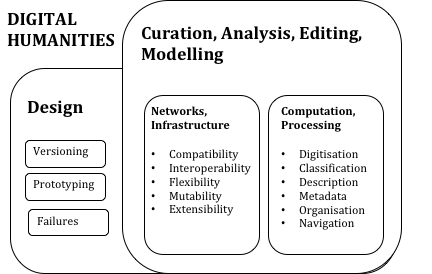
\includegraphics{images/dh01.png}
    \caption[Digital Humanities]{Digital Humanities model}
  \label{fig:Digital_Humanities}
  \end{figure}

  \subsubsection*{NETWORKS, INFRASTRUCTURE}
  \begin{quote}
    Designing and building digital projects depend on knowledge of these fundamentals and on a nuanced understanding of the net- worked environments in which the projects will develop and variously reside. \autocite[p.17]{Burdick2012}
  \end{quote}

  \begin{quote}
    Digital work takes place in the real world, and humanists once accus- tomed to isolated or individualized modes of production must now grapple with complex partnerships and with insuring the long-term availability and viability of their scholarship \autocite[p.21]{Burdick2012}
  \end{quote}

  \subsubsection*{VERSIONING, PROTOTYPING, FAILURES}
  \begin{quote}
    one of the strongest attributes of the field is that the iterative versioning of digital projects fosters experimentation, risk-taking, redefinition, and sometime failure. \autocite[p.21]{Burdick2012}
  \end{quote}

  \begin{draft}
    SOUNDS LIKE SOFTWARE ENGINEERING
  \end{draft}

  \begin{quote}
    It is important that we do not short-circuit this experimental process in the rush to normalize practices, standardize methodologies, and define evaluative metrics. \autocite[p.21]{Burdick2012}
  \end{quote}

  \begin{draft}
    argument for creative computing too
  \end{draft}

  \subsubsection*{Field map of digital humanities: emerging methods and genres}\autocite[p.29-60]{Burdick2012}

  \begin{alltt}
  •	enhanced critical curation
  o	digital collections
  o	multimedia critical editions
  o	object-based argumentation
  o	expanded publication
  o	experiential and spatial
  o	mixed physical and digital
  •	augmented editions and fluid textuality
  o	structured mark-up
  o	natural language processing
  o	relational rhetoric
  o	textual analysis
  o	variants and versions
  o	mutability
  •	scale: the law of large numbers
  o	quantitative analysis
  o	text-mining
  o	machine reading
  o	digital cultural record
  o	algorithmic analysis
  •	distant/close, macro/micro, surface/depth
  o	large-scale patterns
  o	fine-grained analysis
  o	close reading
  o	distant reading
  o	differential geographies
  •	cultural analytics, aggregation, and data-mining
  o	parametrics
  o	cultural mash-ups
  o	computational processing
  o	composite analysis
  o	algorithm design
  •	visualization and data design
  o	data visualization
  o	mapping
  o	information design
  o	simulation environments
  o	spatial argument
  o	modelling knowledge
  o	visual interpretation
  •	locative investigation and thick mapping
  o	spatial humanities
  o	digital cultural mapping
  o	interconnected sites
  o	experimental navigation
  o	geographic information systems (GIS)
  o	stacked data
  •	the animated archive
  o	user communities
  o	permeable walls
  o	active engagement
  o	bottom-up curation
  o	multiplied access
  o	participatory content creation
  •	distributed knowledge production and performative access
  o	global networks
  o	ambient data
  o	collaborative authorship
  o	interdisciplinary teams
  o	use as performance
  o	crowd-sourcing
  •	humanities gaming
  o	user engagement
  o	rule-based play
  o	rich interaction
  o	virtual learning environments
  o	immersion and simulation
  o	narrative complexity
  •	code, software, and platform studies
  o	narrative structures
  o	code as text
  o	computational processes
  o	software in a cultural context
  o	encoding practices
  •	database documentaries
  o	variable experience
  o	user-activated
  o	multimedia prose
  o	modular and combinatoric
  o	multilinear
  •	repurposable content and remix culture
  o	participatory Web
  o	read/write/rewrite
  o	platform migration
  o	sampling and collage
  o	meta-medium
  o	inter-textuality
  •	pervasive infrastructure
  o	extensible frameworks
  o	heterogeneous data streams
  o	polymorphous browsing
  o	cloud computing
  •	ubiquitous scholarship
  o	augmented reality
  o	web of things
  o	pervasive surveillance and tracking
  o	ubiquitous computing
  o	deterritorialization of humanistic practice
  \end{alltt}

  \begin{draft}
    quantifiable and repeatable phenomena versus complex dynamics of interpretation, cultural meanings, probabilistic modelling, interpretive mapping, subjective visualizations, and self-customizing navigation \autocite[p.103]{Burdick2012}
  \end{draft}

  \subsubsection*{TOOLS}
  \begin{quote}
    Building tools around core humanities concepts: subjectivity, ambiguity, contingency, observer-dependent variables in the production of knowledge: holds the promise of expanding current models of knowledge. As such, the next generation of digital experimenters could contribute to humanities theory by forging tools that quite literally embody humanities centred views regarding the world. \autocite[p.104]{Burdick2012}
  \end{quote}

  \begin{quote}
    Tools are not just tools. They are cognitive interfaces that presuppose forms of mental and physical discipline and organization. By scripting an action, they produce and transmit knowledge, and, in turn, model a world. \autocite[p.105]{Burdick2012}
  \end{quote}

  \begin{quote}
    For all its potential interest, a humanities-centered computational environment could well end up distancing humanistic work from the mainstream of digital society, either because of its specialized or speculative character, or because the values that inform its architecture are at odds with the needs of business for standardization, quantitative metrics, and disambiguation. \autocite[p.105]{Burdick2012}
  \end{quote}

  \begin{shaded}
  Summary\\
  •	Collaborative, Transdisciplinary and Computing
  \end{shaded}
\end{draft}


\section{Transdisciplinary}

Basarab Nicolescu distinguished between three different kinds of research `without stable boundaries between the disciplines'.\footnote{Nicolescu cites Jean Piaget here, who first coined the term `transdisciplinarity' in 1972.} \autocite{Nicolescu2010}.

\begin{description}
  \item [Multidisciplinarity]	concerns itself with studying a research topic in not just one discipline but in several simultaneously.
  \item [Interdisciplinarity]	concerns the transfer of methods from one discipline to another.
  \item [Transdisciplinarity]	concerns that which is at once between the disciplines, across the different disciplines, and beyond all disciplines.
\end{description}

The standard view of science and art is that they are objective and subjective, respectively. So, what does that mean for research conducted between, across and beyond science and art, i.e. research that is transdisciplinary?

Nicolescu criticises the view that science must be objective. He even claims that any non-scientific knowledge is `cast into the inferno of subjectivity, tolerated at most as a meaningless embellishment or rejected with contempt as a fantasy, an illusion, a regression, or a product of the imagination' \autocite{Nicolescu2010}. Objectivity\marginnote{§~\ref{ch:pataphysics}}, he says, becomes the `supreme criterion of Truth'\footnote{As we shall see later, pataphysics does the opposite: it reveres the Subject.}

\begin{quotation}
  The death of the Subject is the price we pay for objective knowledge. \sourceatright{\autocite{Nicolescu2010}}
\end{quotation}

He goes on to quote Werner Heisenberg on the concepts of objective and subjective reality: `we would make a very crude simplification if we want to divide the world in[to] one objective reality and one subjective reality. Many rigidities of the philosophy of the last centuries are born by this black and white view of the world.' \autocite[Heisenberg, cited in][]{Nicolescu2010}

\begin{quotation}
  The too strong insistence on the difference between scientific knowledge and artistic knowledge comes from the wrong idea that concepts describe perfectly the ``real things''. […] All true philosophy is situated on the threshold between science and poetry. \sourceatright{\autocite[Heisenberg, cited in][p.22]{Nicolescu2010} \footnote{The full paragraph is worth quoting: `The overly forceful insistence on the difference between scientific and artistic cognition quite likely derives from the incorrect notion that concepts are firmly attached to ``real objects'', as if words had a completely clear and definite meaning in their relationship to reality and as if an accurate sentence, constructed from those words, could deliver an intended ``objective'' factual situation to a more or less absolute degree. But we know, after all, that language too only grasps and shapes reality by turning it into ideas, by idealizing it. Language, too, approaches reality with specific mental forms about which we do not know right away which part of reality they can comprehend and shape. The question about ``right'' or ``wrong'' may indeed be rigorously posed and settled within an idealization, but not in relation to reality. That is why the last measure available for scientific knowledge as well is only the degree to which that knowledge is able to illuminate reality or, better, how that illumination allows us `to find our way' better. And who could question that the spiritual content of a work of art too illumines reality for us and makes it translucent? One must come to terms with the fact that only through the process of cognition itself can we determine what we are to understand by ``cognition''. That is why any genuine philosophy, too, stands on the threshold between science and poetry.' \autocite[Section 2, Chapter 6b]{Heisenberg1942}}}
\end{quotation}

In transdisciplinarity traditional disciplinary boundaries have no meaning. Objectivity is a myth.

\begin{fcom}
  Subject --- Object\\
  subjective --- objective
\end{fcom}

\todo{create figure - subjective vs objective spectrum}

\begin{figure}[!htbp]
\centering
  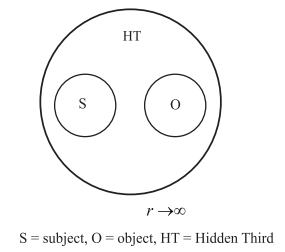
\includegraphics[]{trans}
  \caption[Nicolescu Transdisciplinarity]{Nicolescu Transdisciplinarity}
\label{fig:trans}
\end{figure}

Working across disciplines requires a new unique methodology. Nicolescu proposes a methodology of transdisciplinarity as a non-hierarchical ternary partition of `Subject, Object and Hidden Third'\marginnote{\faicon{object-group}~\ref{fig:trans}} rather than the traditional binary partition of `Subject versus Object'. \autocite{Nicolescu2010}.

% \begin{enumerate}
%   \item \textbf{The ontological axiom}: There are, in Nature and society and in our knowledge of Nature and society, different levels of Reality of the Object and, correspondingly, different levels of Reality of the Subject.
%   \item \textbf{The logical axiom}: The passage from one level of Reality to another is ensured by the logic of the included middle.
%   \item \textbf{The complexity axiom}: The structure of the totality of levels of Reality or perception is a complex structure: every level is what it is because all the levels exist at the same time.
% \end{enumerate}

\begin{quotation}
  The old principle ``unity in diversity and diversity from unity'' is embodied in transdisciplinarity.' \sourceatright{\autocite{Nicolescu2010}}
\end{quotation}

\begin{draft}
  EXplain what exactly i take from this and how this influences my project\\
  why is this more suitable compared to the other methodologies?
\end{draft}

\subsection{Hugill and Yang Methodology}

\begin{quotation}
  `unite and conquer' vs `divide and conquer' \sourceatright{\autocite[p.1]{Yang2013}}
\end{quotation}
\todo{rephrase}

\begin{draft}
  Hugill and Yang suggest that existing research methodologies are unsuitable for transdisciplinary subjects such as \ac{CC}. The following is an example of a possible \ac{CC} research methodology they propose as a starting point \autocite[p.17]{Hugill2013c}:

  \begin{enumerate}
    \item Review literature across disciplines
    \item Identify key creative activities
    \item Analyse the processes of creation
    \item Propose approaches to support these activities and processes
    \item Design and implement software following this approach
    \item Experiment with the resulting system and propose framework
  \end{enumerate}

  They go on to propose four standards for \ac{CC} \autocite[p.17]{Hugill2013c} namely, resist standardisation, perpetual novelty, continuous user interaction and combinational, exploratory and or transformational.
\end{draft}

\begin{draft}

\end{draft}

\subsection{Practice Based}

Linda Candy defines practice based research as follows.

\begin{quotation}
  Practice-based Research is an original investigation undertaken in order to gain new knowledge partly by means of practice and the outcomes of that practice. \sourceatright{\autocite{Candy2006}}
\end{quotation}

She further explains that original contributions to knowledge required in PhD projects can be demonstrated through creative outcomes `in the form of designs, music, digital media, performances and exhibitions' \autocite{Candy2006}.

% \begin{fcom}
%   my practice is software development but framed in arty bollocks.
% \end{fcom}

\todo{finish section on practice based research here}

% \begin{quote}
%   ``Art research is of necessity speculative research. It produces its own protocols; the artist as researcher engages with knowledge in ways that involve the adoption of new frames of reference, the design of new systems and the acquisition of new behaviours. Outcomes will be generally non-linear, associative, connective, transformative and frequently challenging. Trans-disciplinary research in art generates discourse requiring new language.''\autocite[Roy Ascott's preface in][p. v]{Candy2011}
% \end{quote}

% \begin{quote}
%   ``In ways often disconcerting to its academic hosts, art research is prepared to look in all directions for inspiration, understanding and explication: to the East as well as the West, so to speak; following the left-hand path as well as the right; working with both reason and intuition, sense and nonsense, subtelty and sensibility. It is what can be called a transdisciplinary syncretism that best informs artistic research, just as it is the integrative faculty of ‘cyberception’ that enables our focus on mutliple realities and a technoetic instrumentality that supports art strategies involving the evolution of mind, the networked distribution of presence and the re-configuration of personal identity. Art research is second-order research; the researcher is always a part of the system or subject of inquiery. Innovation in subjectivity prevails over odurate objectivity. [...] methodologies that can, whenever needed, put subject before object, process before system, behaviour before form, intuition before reason and mind before matter.''\autocite[Roy Ascott's preface in][p. vi]{Candy2011}
% \end{quote}

\begin{figure}[!htbp] % (here, top, bottom, page)
  \centering
  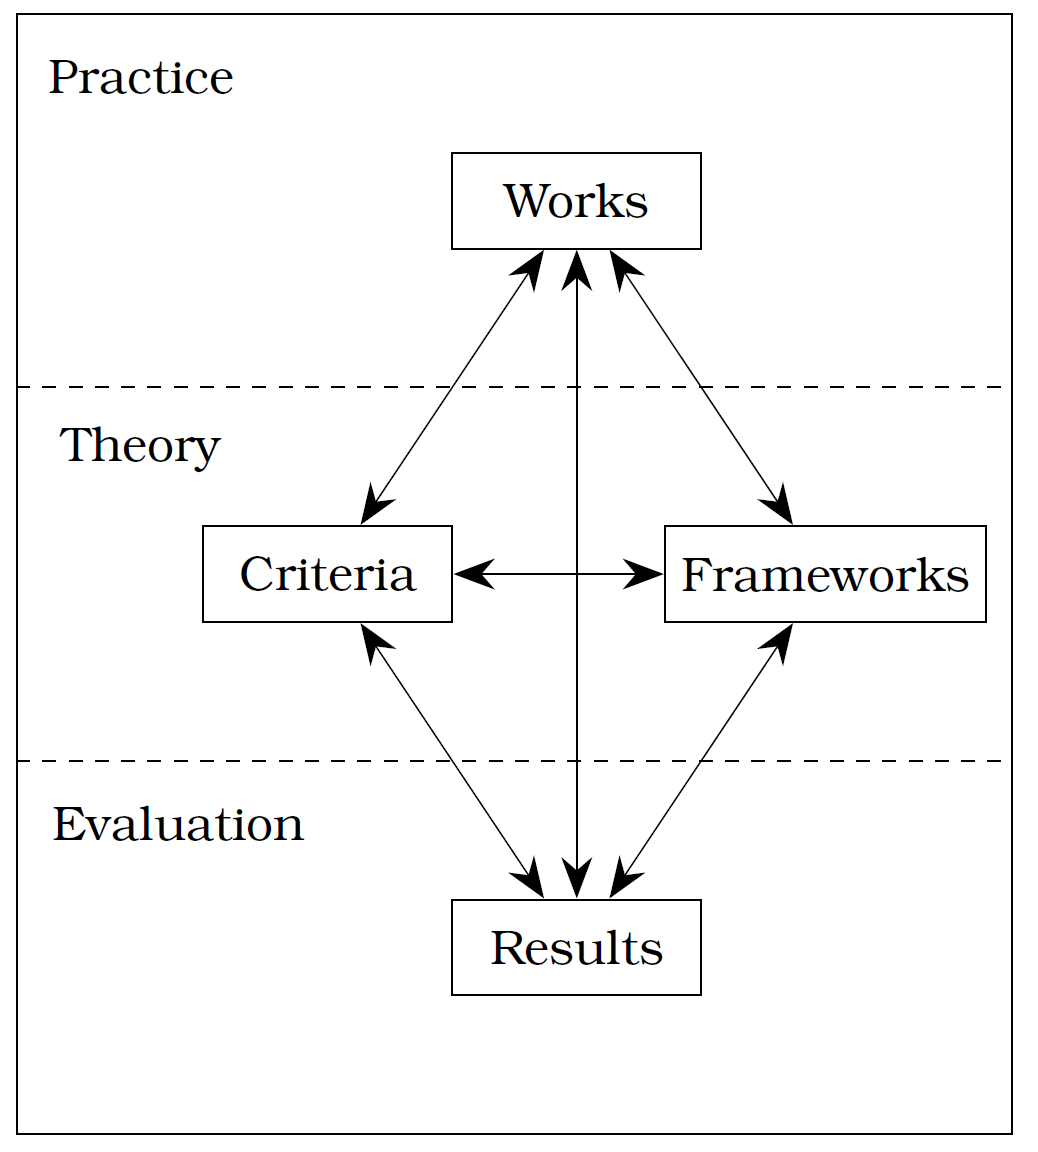
\includegraphics[width=.5\textwidth]{tmpr}
  \caption[Trajectory Model]{Edmonds and Candy's Trajectory Model (W = Works, C = Criteria, F = Frameworks, R = Results)}
\label{fig:tmpr}
\end{figure}

Figure~\ref{fig:tmpr}\marginnote{\faicon{object-group}~\ref{fig:tmpr}} shows the \ac{TMPR} developed by Ernest Edmonds and Linda Candy as a framework to `influence practice, inform theory and, in particular, shape evaluation' \autocite{Edmonds2010}. The model allows for different trajectories between practice, theory and evaluation. Table~\ref{tab:tmpr}\marginnote{\faicon{table}~\ref{tab:tmpr}} shows the various elements, activities and outcomes in this framework more clearly.

\begin{table}[!htbp]
\caption[Elements, Activities and Outcomes of the \ac{TMPR}]{Elements, Activities and Outcomes of each Trajectory in the \ac{TMPR}}
\label{tab:tmpr}
  \begin{tabu}{X[1]X[2]X[3]}
  \toprule
  \textbf{Elements}
  &
  \textbf{Activities}
  &
  \textbf{Outcomes}
  \\ \midrule
  \textbf{Practice}
  &
  create, exhibit, reflect
  &
  \textbf{Works:} consisting of physical artefacts, musical compositions, software systems, installations, exhibitions, collaborations
  \\ \midrule
  \textbf{Theory}
  &
  read, think, write, develop
  &
  \textbf{Frameworks:} comprising questions, criteria, issues
  \\ \midrule
  \textbf{Evaluation}
  &
  observe, record, analyse, reflect
  &
  \textbf{Results:} findings leading to new/modified Works and Frameworks
  \\ \bottomrule
  \end{tabu}
\end{table}


\section{My Research Approach}
\label{s:mymeth}

\todo{rapid incremental prototyping}

The doctoral research presented in this thesis does not fit into neat categories in science or art---making it transdisciplinary in nature. Subjects like literature, philosophy, cognitive science, artificial intelligence, software engineering and linguistics frame the three core areas of research for this project, namely pataphysics, creativity and computing.

To address the transdisciplinary nature of the project I 


employed a practice-based research methodology, meaning that part of my submission for the degree of Doctor of Philosophy is an artefact demonstrating my original contribution to knowledge. The thesis provides the context of this artefact and critically analyses and discusses the experimental process and outcome.

\begin{description}
  \item [Epistemology] Transdisciplinary, Subjective
  \item [Methodology] Qualitative, Exploratory
  \item [Methods] Creative Computing, Website Development, Literature Review, Evaluation Framework, Critical Reflection
\end{description}

The general workflow of my project was as follows.
\begin{draft}
relates back to hugill and yang approach
\end{draft}

\begin{enumerate}
  \item Conduct extensive literature review into the various subjects involved,
  \item develop pataphysical algorithms,
  \item develop an evaluation framework,
  \item design a system to demonstrate algorithms,
  \item develop a website for the tool,
  \item evaluate website using framework and redevelop as needed and
  \item write up findings.
\end{enumerate}

In regards to the practice based methodology, I followed the following trajectory inspired by the \ac{TMPR}\marginnote{\faicon{object-group}~\ref{fig:tmpr}}.

\todo{create my own tmpr figure here}

\begin{description}
  \item [Practice] (Works): Implementation of Algorithms, Development of Website
  \item [Theory] (Criteria, Frameworks): Creation of Algorithms, Setting Context, Define Evaluation Framework
  \item [Evaluation] (Results): Interpretation of Work
\end{description}

\begin{draft}
  This tmpr is my thesis.\\
  works: pata.physics.wtf\\
  criteria: criteria for creativity\\
  frameworks: evaluation framework\\
  results: conclusion
\end{draft}

\begin{draft}
  does the tpmr fit into the hugill and yang approach?
\end{draft}



The general process\marginnote{§~\ref{ch:implementation}} of my project was as follows.

\begin{enumerate}
  \item Conduct extensive literature review into the various subjects involved,
  \item develop pataphysical algorithms,
  \item develop an evaluation framework,
  \item design a system to demonstrate algorithms,
  \item develop a website for the tool,
  \item evaluate website using framework and redevelop as needed and
  \item write up findings.
\end{enumerate}


\todo{comp creat vs creat comp}
\begin{draft}
  list out the different examples of why my project is both of the above. 
  eg it is comp creat because i use javascript+maths for display the poetry
  but creat comp is the mis-use of damerau levensthein algorithm
\end{draft}


\stopcontents[chapters]
